\documentclass[pdflatex,sn-mathphys]{sn-jnl}
\jyear{\year}

\usepackage{lipsum}

\raggedbottom

\begin{document}

\title[Modelagem de processo industrial de manufatura]{Modelagem de processo industrial de manufatura}

%\author*[1,2]{\pfx{Dr} \fnm{Joergen W.} \spfx{van der} \sur{Ploeg} \sfx{IV} \tanm{Poet Laureate} \dgr{MSc, PhD}}\email{iauthor@gmail.com}

\author[1]{\fnm{First} \sur{Author}}\email{iauthor@gmail.com}

\author[1]{\fnm{ii} \sur{Author}}\email{iiauthor@gmail.com}

\author[1]{\fnm{iii} \sur{Author}}\email{iiiauthor@gmail.com}

\affil[1]{\orgdiv{Programa de Pós-Graduação em Engenharia Elétrica}, \orgname{Universidade Tecnológica Federal do Paraná}, \orgaddress{\street{Via do Conhecimento}, \city{Pato Branco}, \postcode{85503-390}, \state{PR}, \country{Brasil}}}

\abstract{\lipsum[1-2]}

\keywords{SEDs, Industry 4.0, TCS}

\maketitle

\section{Introdução}

Este trabalho aborda o desenvolvimento de um controle supervisório para uma planta industrial com processo de  manufatura. A figura \ref{fig:processo} apresenta uma visão da planta industrial a ser modelada e simulada.

%\subsection{Processo industrial de manufatura}

\begin{figure}[H]%
	\centering
	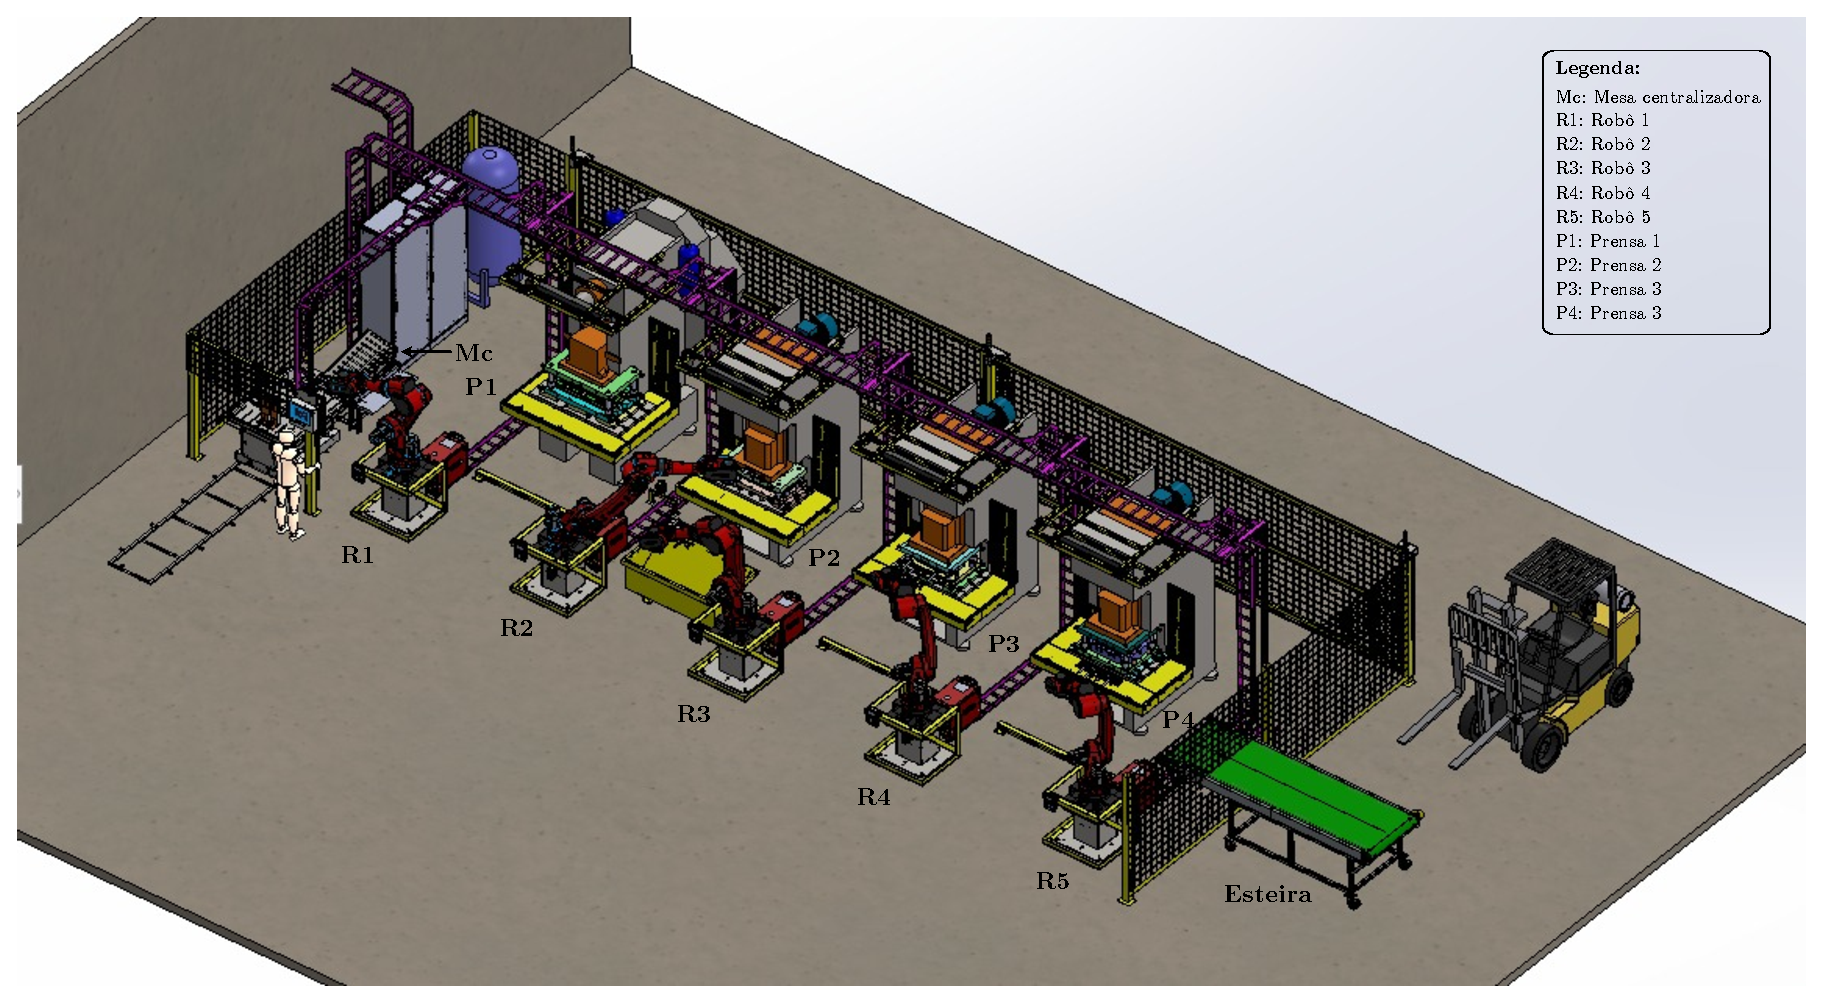
\includegraphics[width=0.8\textwidth]{imagens/processo.eps}
	\caption{Planta industrial}\label{fig:processo}
\end{figure}

A planta é composta por:
\begin{itemize}
    \item Mesa centralizadora com teste de chapa;
    \item 5 robôs manipuladores;
    \item 4 prensas;
    \item Esteira para destinação final das peças;
\end{itemize}

Partindo de uma posição segura para todos os robôs, o primeiro robô inicia sua movimentação para pegar a chapa da mesa centralizadora e levar até a primeira prensa, ao finalizar o processo o segundo robô faz o transporte até a segunda prensa e assim sucessivamente até o robô 4, que entrega a peça ao robô 5 e esse insere na ultima prensa e realiza a entrega o produto pronto para a esteira. 

No caso de uma interrupção o sistema retorna a uma condição inicial em que todos robôs retornam a posição de segurança, estão livre de peças e as prensas ficam livres de peças e no ponto morto superior. Um operador, se necessário manualmente fará o controle do robô para a retirada de peças que estejam no meio do processo e voltar a posição de segurança para um recomeço da linha de manufatura, isso ocorre pois ele perde a referência de localização, justificando o \textit{reset} de todos os elementos.

O controle modular será aplicado dada a possibilidade de tratar individualmente cada etapa do conjunto descentralizando em subplantas e especificações locais, formando os supervisores locais. Se não conflitarem entre si, irão compor um supervisor completo com comportamento equivalente a um supervisor monolítico.
%\section{Revisão}
\section{Modelos projetados}
\subsection{Plantas}
Robôs 1 e 2

TODO: descrição do funcionamento dos robôs

\begin{figure}[H]%
  \centering
  \begin{subfigure}[b]{0.45\textwidth}
      \centering
      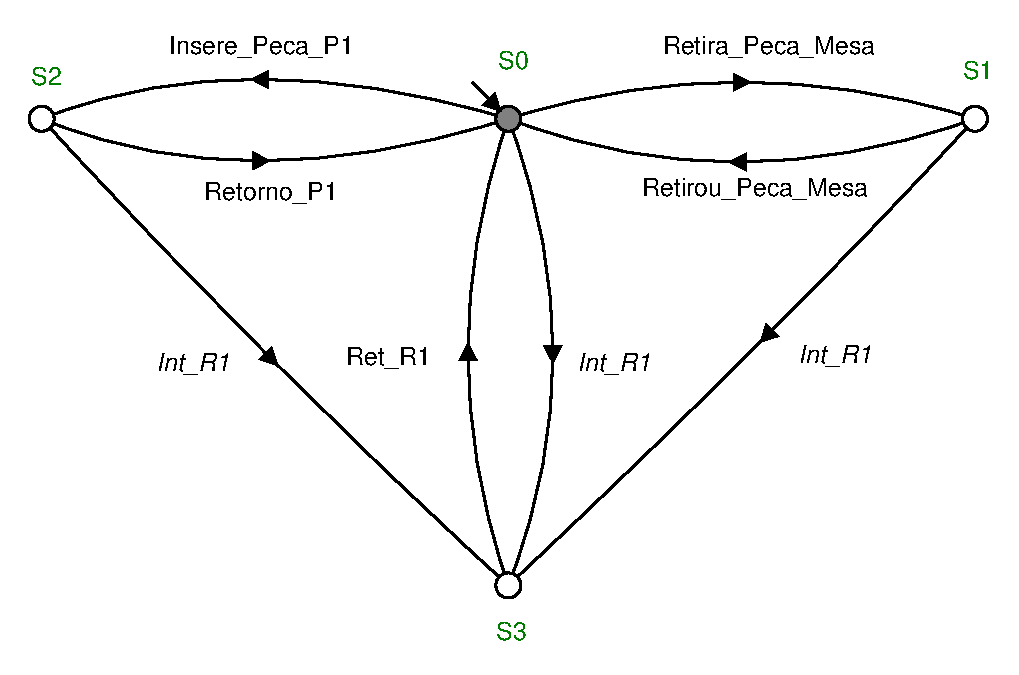
\includegraphics[width=\textwidth]{imagens/Robo_1.eps}
      \caption{Robô 1}
      \label{fig:r1}
  \end{subfigure}
  \hfill
  \begin{subfigure}[b]{0.45\textwidth}
      \centering
      \includegraphics[width=\textwidth]{imagens/Robo_2.eps}
      \caption{Robô 2}
      \label{fig:r2}
  \end{subfigure}
  \caption{Planta Robôs 1 e 2}
  \label{fig:robo12}
\end{figure}

Robôs 3 e 4

TODO: descrição do funcionamento dos robôs

\begin{figure}[H]%
  \centering
  \begin{subfigure}[b]{0.45\textwidth}
      \centering
      \includegraphics[width=\textwidth]{imagens/Robo_3.eps}
      \caption{Robô 3}
      \label{fig:r3}
  \end{subfigure}
  \hfill
  \begin{subfigure}[b]{0.45\textwidth}
      \centering
      \includegraphics[width=\textwidth]{imagens/Robo_4.eps}
      \caption{Robô 4}
      \label{fig:r4}
  \end{subfigure}
  \caption{Planta Robôs 3 e 4}
  \label{fig:robo34}
\end{figure}

Robô 5

TODO: descrição do funcionamento do robô

\begin{figure}[H]%
    \centering
    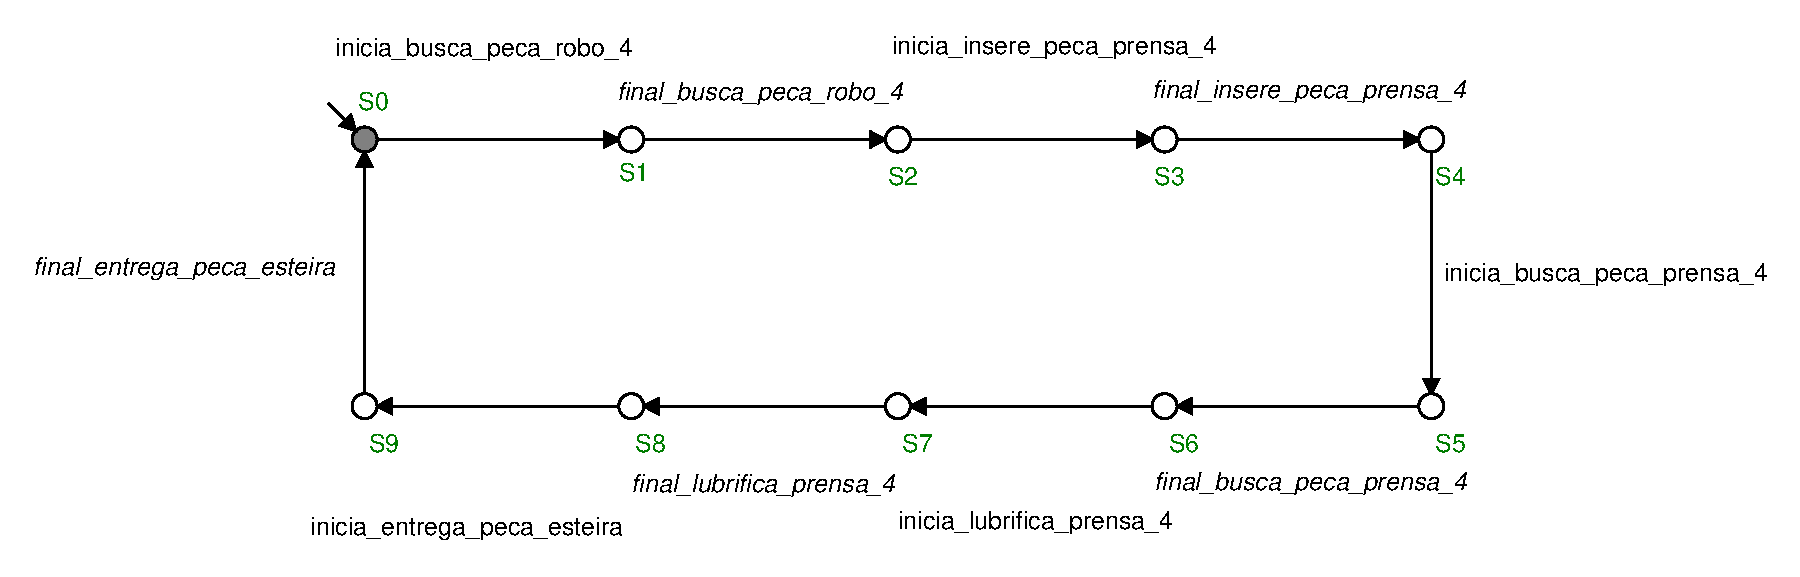
\includegraphics[width=0.9\textwidth]{imagens/robo_5.eps}
    \caption{Planta Robô 3}\label{fig:robo5}
\end{figure}

Todas as prensas têm o mesmo modelo, a seguir apresenta-se o modelo genérico para as prensas.

TODO: descrever funcionamento esperado para uma prensa, talvez.

\begin{figure}[H]%
    \centering
    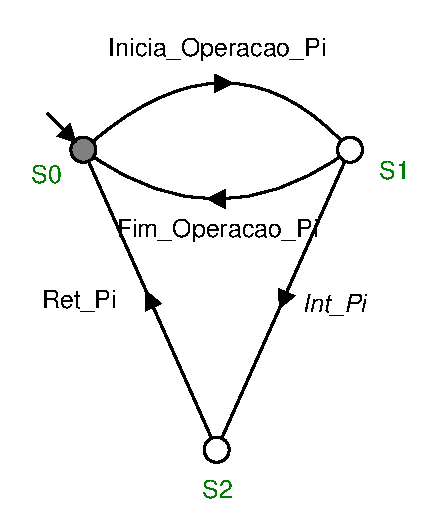
\includegraphics[width=0.6\textwidth]{imagens/Prensa.eps}
    \caption{Planta Prensa}\label{fig:prensa}
\end{figure}

\subsection{Especificações}
A seção a seguir são apresenta as especificações desenvolvidas para cumprir com os requisitos de controle desejados.

A especificação apresentada na Figura \ref{fig:e0} permite ao Robô 1 retirar peças da mesa centralizadora após o sensor detectar existencia de peça sobre a mesa.
Já a especificação apresentada na Figura \ref{fig:e1} limita o Robô 1 a iniciar o processo de inserção na Prensa 1 após ter peça presente na garra.

\begin{figure}[H]%
  \centering
  \begin{subfigure}[b]{0.45\textwidth}
      \centering
      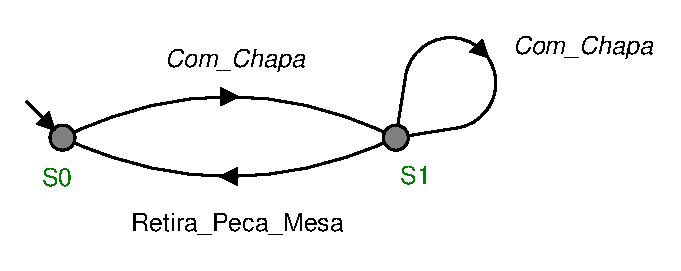
\includegraphics[width=\textwidth]{imagens/E0.eps}
      \caption{E0}
      \label{fig:e0}
  \end{subfigure}
  \hfill
  \begin{subfigure}[b]{0.45\textwidth}
      \centering
      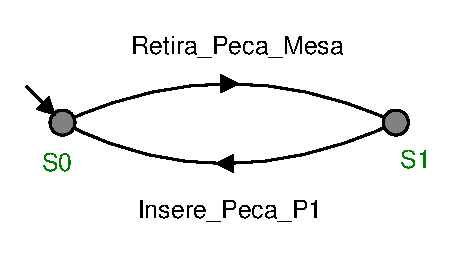
\includegraphics[width=\textwidth]{imagens/E1.eps}
      \caption{E1}
      \label{fig:e1}
  \end{subfigure}
  \caption{Especificações 0 e 1}
  \label{fig:e01}
\end{figure}

A especificação apresentada na Figura \ref{fig:e2} permite que a Prensa 1 inicie a operação após o Robô 1 finalizar a inserção e estar em posição segura.
Já a especificação apresentada na \ref{fig:e3} é o modelo para overflow da Prensa 1 e libera uma nova inserção após a retirada da peça pelo Robô 2.

\begin{figure}[H]%
  \centering
  \begin{subfigure}[b]{0.45\textwidth}
      \centering
      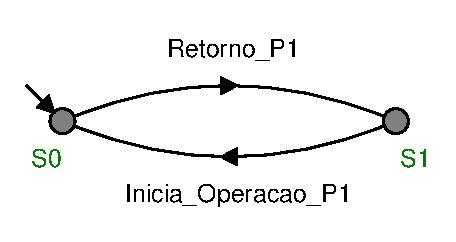
\includegraphics[width=\textwidth]{imagens/E2.eps}
      \caption{E2}
      \label{fig:e2}
  \end{subfigure}
  \hfill
  \begin{subfigure}[b]{0.45\textwidth}
      \centering
      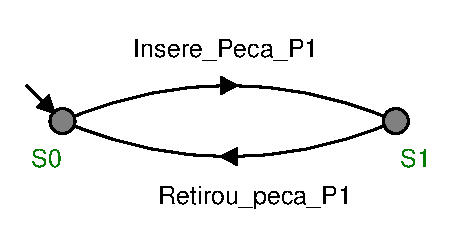
\includegraphics[width=\textwidth]{imagens/E3.eps}
      \caption{E3}
      \label{fig:e3}
  \end{subfigure}
  \caption{Especificações 2 e 3}
  \label{fig:e23}
\end{figure}

A especificação apresentada na Figura \ref{fig:e4} limita o Robô 2 a retirar peça da Prensa 1 após o final da operação.
Já a especificação apresentada na \ref{fig:e5} limita o Robô 2 a iniciar o processo de inserção na Prensa 2 após ter peça presente na garra.

\begin{figure}[H]%
  \centering
  \begin{subfigure}[b]{0.45\textwidth}
      \centering
      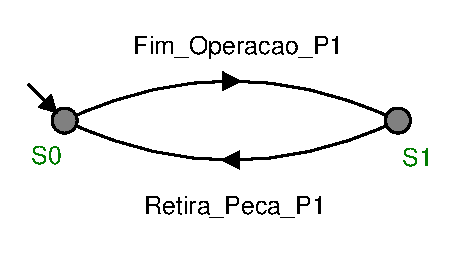
\includegraphics[width=\textwidth]{imagens/E4.eps}
      \caption{E4}
      \label{fig:e4}
  \end{subfigure}
  \hfill
  \begin{subfigure}[b]{0.45\textwidth}
      \centering
      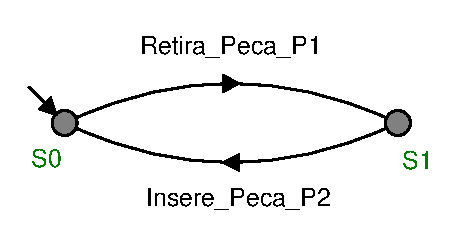
\includegraphics[width=\textwidth]{imagens/E5.eps}
      \caption{E5}
      \label{fig:e5}
  \end{subfigure}
  \caption{Especificações 4 e 5}
  \label{fig:e45}
\end{figure}

A especificação apresentada na Figura \ref{fig:e6} permite que a Prensa 2 inicie a operação após o Robô 2 finalizar a inserção e estar em posição segura.
Já a especificação apresentada na \ref{fig:e7} é o modelo para overflow da Prensa 2 e libera uma nova inserção após a retirada da peça pelo Robô 3.

\begin{figure}[H]%
  \centering
  \begin{subfigure}{0.45\textwidth}
      \centering
      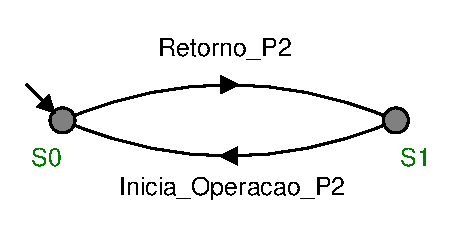
\includegraphics[width=\textwidth]{imagens/E6.eps}
      \caption{E6}
      \label{fig:e6}
  \end{subfigure}
  \hfill
  \begin{subfigure}{0.45\textwidth}
      \centering
      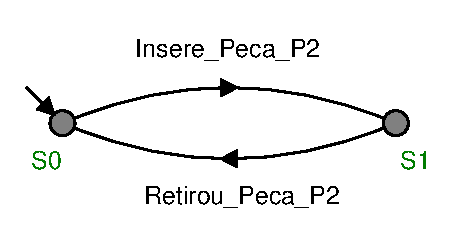
\includegraphics[width=\textwidth]{imagens/E7.eps}
      \caption{E7}
      \label{fig:e7}
  \end{subfigure}
  \caption{Especificações 6 e 7}
  \label{fig:e67}
\end{figure}

A especificação apresentada na Figura \ref{fig:e8} limita o Robô 3 a retirar peça da Prensa 2 após o final da operação.
Já a especificação apresentada na \ref{fig:e9} limita o Robô 3 a iniciar o processo de inserção na Prensa 3 após ter peça presente na garra..

\begin{figure}[H]%
  \centering
  \begin{subfigure}{0.45\textwidth}
      \centering
      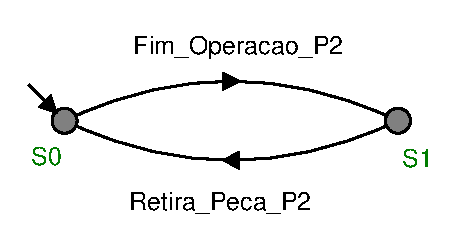
\includegraphics[width=\textwidth]{imagens/E8.eps}
      \caption{E8}
      \label{fig:e8}
  \end{subfigure}
  \hfill
  \begin{subfigure}{0.45\textwidth}
      \centering
      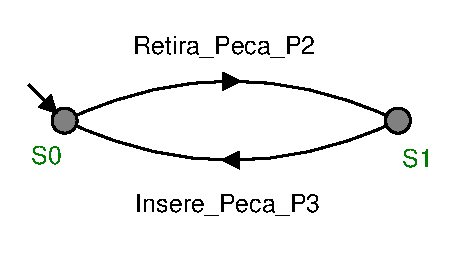
\includegraphics[width=\textwidth]{imagens/E9.eps}
      \caption{E9}
      \label{fig:e9}
  \end{subfigure}
  \caption{Especificações 8 e 9}
  \label{fig:e89}
\end{figure}

A especificação apresentada na Figura \ref{fig:e10} permite que a Prensa 3 inicie a operação após o Robô 3 finalizar a inserção e estar em posição segura.
Já a especificação apresentada na \ref{fig:e11} é o modelo para overflow da Prensa 3 e libera uma nova inserção após a retirada da peça pelo Robô 4.

\begin{figure}[H]%
  \centering
  \begin{subfigure}{0.45\textwidth}
      \centering
      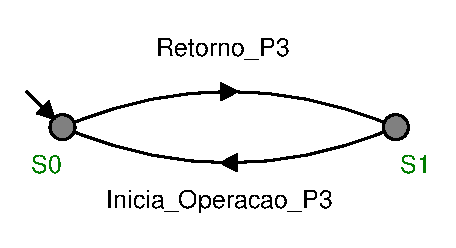
\includegraphics[width=\textwidth]{imagens/E10.eps}
      \caption{E10}
      \label{fig:e10}
  \end{subfigure}
  \hfill
  \begin{subfigure}{0.45\textwidth}
      \centering
      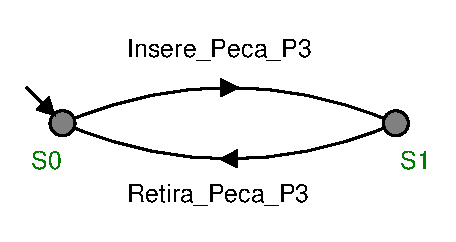
\includegraphics[width=\textwidth]{imagens/E11.eps}
      \caption{E11}
      \label{fig:e11}
  \end{subfigure}
  \caption{Especificações 10 e 11}
  \label{fig:e1011}
\end{figure}

A especificação apresentada na Figura \ref{fig:e12} limita o Robô 4 a retirar peça da Prensa 3 após o final da operação.
Já a especificação apresentada na \ref{fig:e13} limita o Robô 4 a iniciar o processo de entrega para Robô 5 após ter peça presente na garra.

\begin{figure}[H]%
  \centering
  \begin{subfigure}{0.45\textwidth}
      \centering
      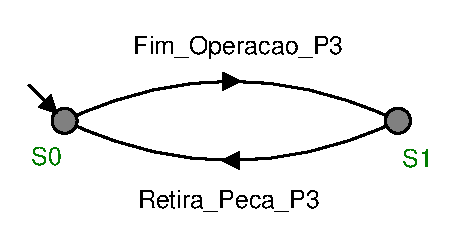
\includegraphics[width=\textwidth]{imagens/E12.eps}
      \caption{E12}
      \label{fig:e12}
  \end{subfigure}
  \hfill
  \begin{subfigure}{0.45\textwidth}
      \centering
      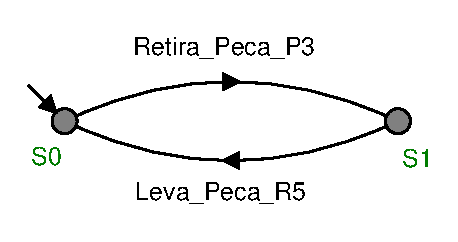
\includegraphics[width=\textwidth]{imagens/E13.eps}
      \caption{E13}
      \label{fig:e13}
  \end{subfigure}
  \caption{Especificações 12 e 13}
  \label{fig:e1213}
\end{figure}

A especificação apresentada na Figura \ref{fig:e14} permite que a Prensa 4 inicie a operação após o Robô 5 finalizar a inserção e estar em posição segura.
Já a especificação apresentada na \ref{fig:e15} limita o Robô 5 a retirar peça da Prensa 5 após o final da operação.

\begin{figure}[H]%
  \centering
  \begin{subfigure}{0.45\textwidth}
      \centering
      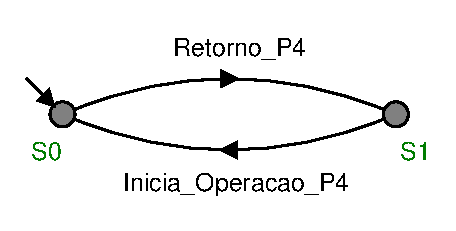
\includegraphics[width=\textwidth]{imagens/E14.eps}
      \caption{E14}
      \label{fig:e14}
  \end{subfigure}
  \hfill
  \begin{subfigure}{0.45\textwidth}
      \centering
      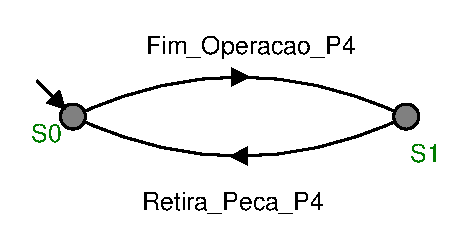
\includegraphics[width=\textwidth]{imagens/E15.eps}
      \caption{E15}
      \label{fig:e15}
  \end{subfigure}
  \caption{Especificações 14 e 15}
  \label{fig:e1415}
\end{figure}

A especificação apresentada na Figura \ref{fig:e16} força Robô 4 ao entregar uma peça aguarde o movimento do Robô 5 de buscar a peça.
Já a especificação apresentada na \ref{fig:e17} força o Robô 4 a aguardar posição segura do Robô 5 para retornar do movimento de entrega de peça.

\begin{figure}[H]%
  \centering
  \begin{subfigure}{0.45\textwidth}
      \centering
      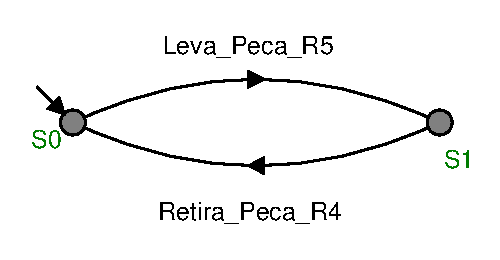
\includegraphics[width=\textwidth]{imagens/E16.eps}
      \caption{E16}
      \label{fig:e16}
  \end{subfigure}
  \hfill
  \begin{subfigure}{0.45\textwidth}
      \centering
      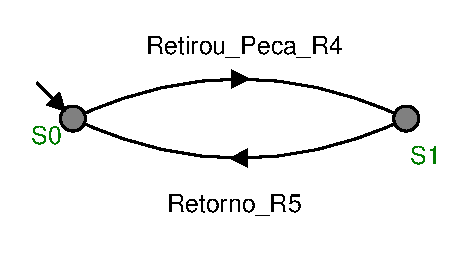
\includegraphics[width=\textwidth]{imagens/E17.eps}
      \caption{E17}
      \label{fig:e17}
  \end{subfigure}
  \caption{Especificações 16 e 17}
  \label{fig:e1617}
\end{figure}

A especificação apresentada na Figura \ref{fig:e18} limita o Robô 5 a iniciar o processo de inserção na Prensa 4 após ter peça presente na garra.
Já a especificação apresentada na \ref{fig:e19} permite que o Robô 5 pegue uma nova peça do Robô 4 após entregar a peça manufaturada na esteira.

\begin{figure}[H]%
  \centering
  \begin{subfigure}{0.45\textwidth}
      \centering
      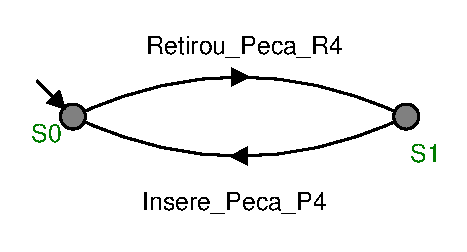
\includegraphics[width=\textwidth]{imagens/E18.eps}
      \caption{E18}
      \label{fig:e18}
  \end{subfigure}
  \hfill
  \begin{subfigure}{0.45\textwidth}
      \centering
      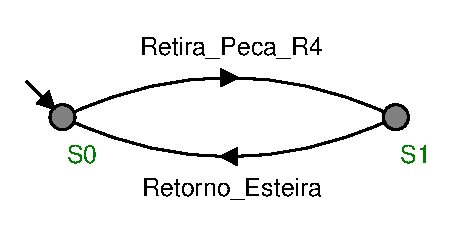
\includegraphics[width=\textwidth]{imagens/E19.eps}
      \caption{E19}
      \label{fig:e19}
  \end{subfigure}
  \caption{Especificações 18 e 19}
  \label{fig:e1819}
\end{figure}

\subsection{Solução modular de controle}
O software Supremica \cite{Supremica2020} disponibiliza funcionalidade para verificação da modularidade dos modelos desenvolvidos.
A Figura \ref{fig:modulare0} apresenta o resultado da análise da modularidade da especificação E0 com as plantas, podemos verificar que a especificação realiza controle de eventos sobre o Robô 1 e sobre Sensor Chapa sem ter dependencia com outras plantas.

\begin{figure}[H]%
  \centering
  \includegraphics[width=0.8\textwidth]{imagens/modular_E0.eps}
  \caption{Planta industrial}\label{fig:modulare0}
\end{figure}

O processo de verificação de modularidade foi executado para todas as especificações, a tabela \ref{tab:modulos} apresenta o resultado para cada especificação e as respectivas plantas com atuação.
Foi verificado que o número máximo de interações de uma especificações é com duas plantas.

\begin{table}[h]
\begin{center}
\begin{minipage}{0.5\textwidth}
\caption{Relações entre plantas e especificações}
\label{tab:modulos}
\begin{tabular}{@{}lll@{}}
  \toprule
  Especificação &  Planta 1 & Planta 2\\
  \midrule
  E0 & Sensor Chapa & Robô 1\\
  E1 & Robô 1 & \\
  E2 & Robô 1 & Prensa 1\\
  E3 & Robô 1 & Robô 2\\
  E4 & Robô 2 & Prensa 1\\
  E5 & Robô 2 & \\
  E6 & Robô 2 & Prensa 2\\
  E7 & Robô 2 & Robô 3\\
  E8 & Robô 3 & Prensa 2\\
  E9 & Robô 3 & \\
  E10 & Robô 3 & Prensa 3\\
  E11 & Robô 3 & Robô 4\\
  E12 & Robô 4 & Prensa 3\\
  E13 & Robô 4 & \\
  E14 & Robô 5 & Prensa 4\\
  E15 & Robô 5 & Prensa 4\\
  E16 & Robô 4 & Robo 5\\
  E17 & Robô 4 & Robo 5\\
  E18 & Robô 5 & \\
  E19 & Robô 5 & \\
  \botrule
\end{tabular}
\end{minipage}
\end{center}
\end{table}

A Tabela \ref{tab:supervisor} apresenta o número de estados, transições e eventos para cada supervisor modular e para o supervisor final.

\begin{table}[h]
\begin{center}
\begin{minipage}{0.5\textwidth}
\caption{Supervisores Modulares}
\label{tab:supervisor}
\begin{tabular}{@{}llll@{}}
  \toprule
  Supervisor & Estados & Eventos & Transições\\
  \midrule
  Sup 0 & 6 & 6 & 17\\
  Sup 1 & 6 & 6 & 10\\
  Sup 2 & 24 & 10 & 73\\
  Sup 3 & 32 & 12 & 120\\
  Sup 4 & 24 & 10 & 73\\
  Sup 5 & 6 & 6 & 10\\
  Sup 6 & 24 & 10 & 73\\
  Sup 7 & 32 & 12 & 120\\
  Sup 8 & 24 & 10 & 73\\
  Sup 9 & 6 & 6 & 10\\
  Sup 10 & 24 & 10 & 73\\
  Sup 11 & 32 & 12 & 120\\
  Sup 12 & 24 & 10 & 73\\
  Sup 13 & 6 & 6 & 10\\
  Sup 14 & 30 & 12 & 98\\
  Sup 15 & 30 & 12 & 98\\
  Sup 16 & 40 & 14 & 159\\
  Sup 17 & 40 & 14 & 159\\
  Sup 18 & 9 & 8 & 18\\
  Sup 19 & 9 & 8 & 18\\
  \midrule
  \textbf{Final} & & &\\
  \botrule
\end{tabular}
\end{minipage}
\end{center}
\end{table}
\section{Conclusões}
Após elaborar as plantas e todas as especificações locais, os supervisores locais puderam ser calculados, porém vários retornam um grande número de estados e transições. Ao fazer o produto síncrono para obter o equivalente ao controle monolítico houve uma explosão de estados pelo crescimento exponencial associado à complexidade da síntese modular local.

Logo é sugerido a aplicação de ferramentas que possam reduzir o número de dados, como algoritmos de minimização para os supervisores locais antes de obter o supervisor completo \cite{Queiroz}, ou ainda aplicar o controle utilizando características de mestre e subordinado.

\bibliography{sn-bibliography}

\end{document}
